%
\section{Track reconstruction}
The (P1+P2) distribution for events with two reconstructed tracks is shown in Figure~\ref{figure:t2_1_smom_0}.
No track selection cuts are applied. A $\gamma \to e^+e^-$ peak  is clearly seen.

\begin{figure}[H]
  \begin{tikzpicture}
    \node[anchor=south west,inner sep=0] at (0,0.) {
      % \node[shift={(0 cm,0.cm)},inner sep=0,rotate={90}] at (0,0) {}
      \makebox[\textwidth][c] {
        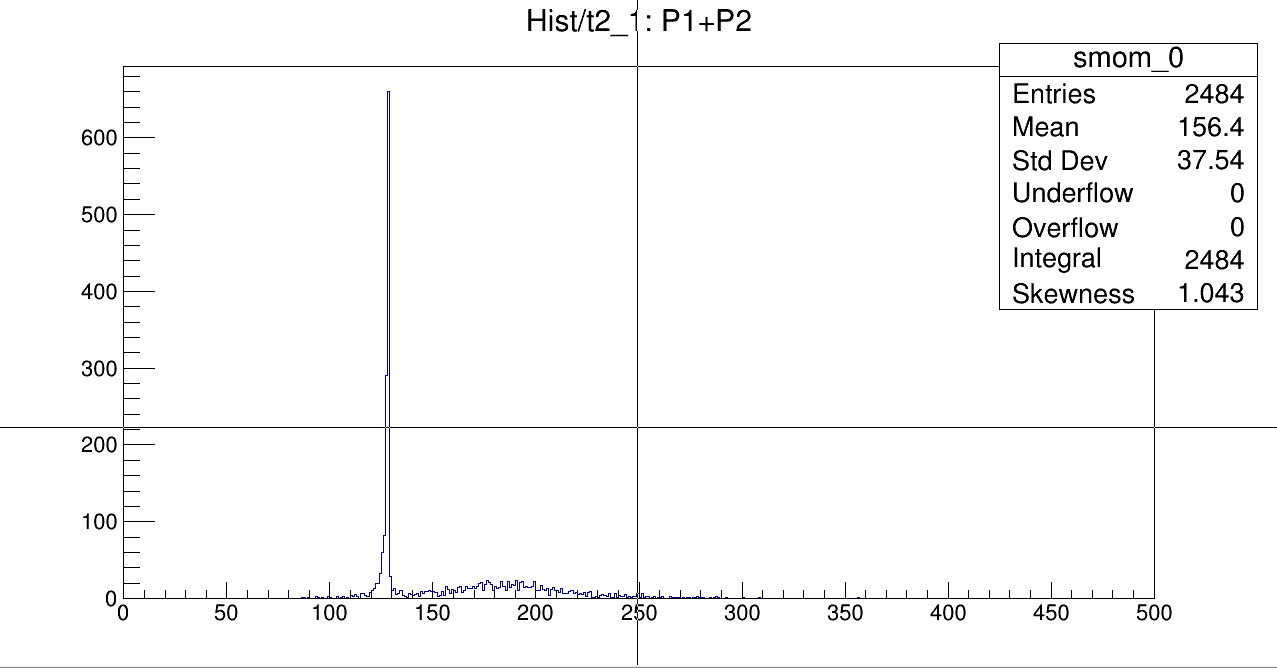
\includegraphics[width=0.95\textwidth]{png/pipenu_bpip4b0s54r0100_murat_drpc_ana_t2_1_smom_0}
      }
    };
    % \node [text width=8cm, scale=1.0] at (14.5,0.5) {$\mu_B$, expected background mean};
    % \node [text width=8cm, scale=1.0, rotate={90}] at (1.5,7.5) { $S_{D}$, ``discovery'' signal strength  };
  \end{tikzpicture}
  \caption{
    \label{figure:t2_1_smom_0}
    Sum of the two reconstructed track momenta
  }
  \label{figure:event_display}
\end{figure}

Figure~\ref{figure:t2_1_smom_1_fit} shows the fit of the conversion peak with the function
defined by \ref{}... The offset of the reconstructed peak due to the energy losses is 1 MeV,
and the peak FWHM is also close to 1 MeV.

Comparison of Figure ~\ref{figure:t2_1_smom_1_fit} to Figure ~\ref{figure:t2_1_smom_1_fit}
gives the reconstruction efficiency for preselected events of about 10\% which is fairly low.

\begin{figure}[H]
  \begin{tikzpicture}
    \node[anchor=south west,inner sep=0] at (0,0.) {
      % \node[shift={(0 cm,0.cm)},inner sep=0,rotate={90}] at (0,0) {}
      \makebox[\textwidth][c] {
        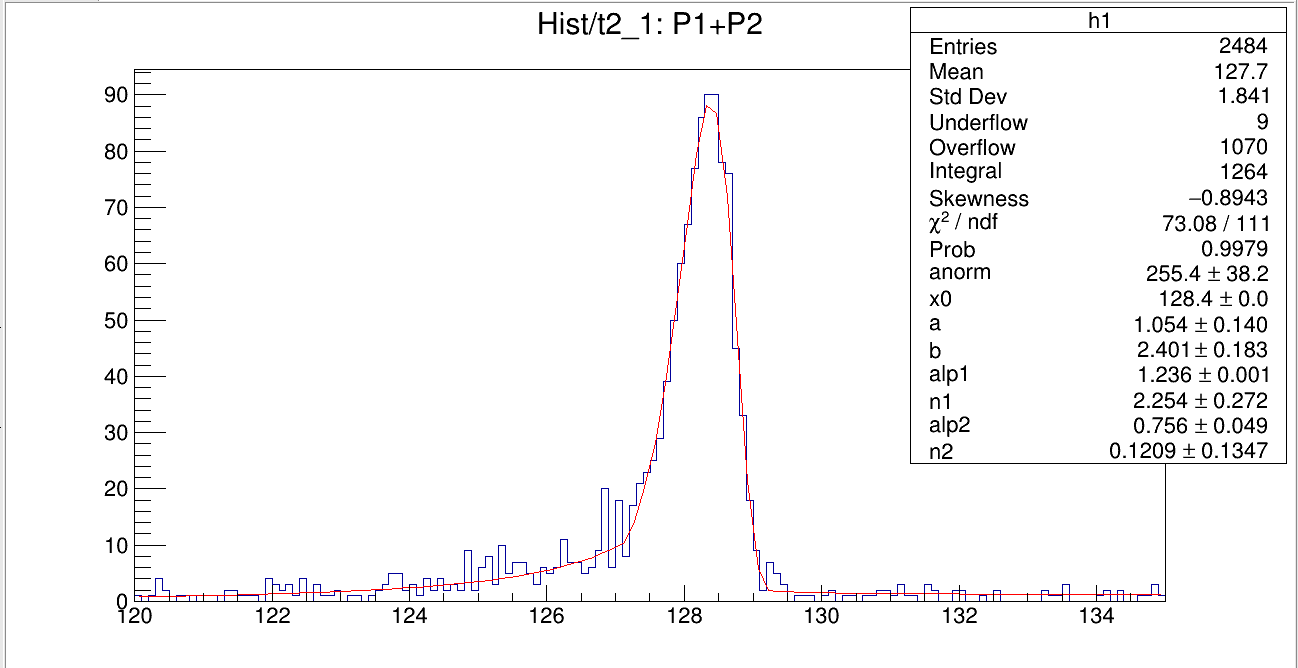
\includegraphics[width=0.95\textwidth]{png/pipenu_bpip4b0s54r0100_murat_drpc_ana_t2_1_smom_1_fit}
      }
    };
    % \node [text width=8cm, scale=1.0] at (14.5,0.5) {$\mu_B$, expected background mean};
    % \node [text width=8cm, scale=1.0, rotate={90}] at (1.5,7.5) { $S_{D}$, ``discovery'' signal strength  };
  \end{tikzpicture}
  \caption{
    \label{figure:t2_1_smom_1_fit}
    Sum of the two reconstructed track momenta
  }
  \label{figure:event_display}
\end{figure}

However the Mu2e track reconstruction, first of all - the pattern recognition, has never
been optimized for low momentum tracks. An example of a misreconstructed $\gamma \to e^+e^-$
event is shown in Figure ~\ref{figure:event_display}. In this event there are two particles,
an electron and a positron entering the tracker with the momenta of 83.7 and 43.5 MeV/c
correspondingly. Only one of them, the 83.7 MeV/c electron, has a reconstructed track, and 
the positron track has not been found.  

\begin{figure}[H]
  \begin{tikzpicture}
    \node[anchor=south west,inner sep=0] at (0,0.) {
      % \node[shift={(0 cm,0.cm)},inner sep=0,rotate={90}] at (0,0) {}
      \makebox[\textwidth][c] {
        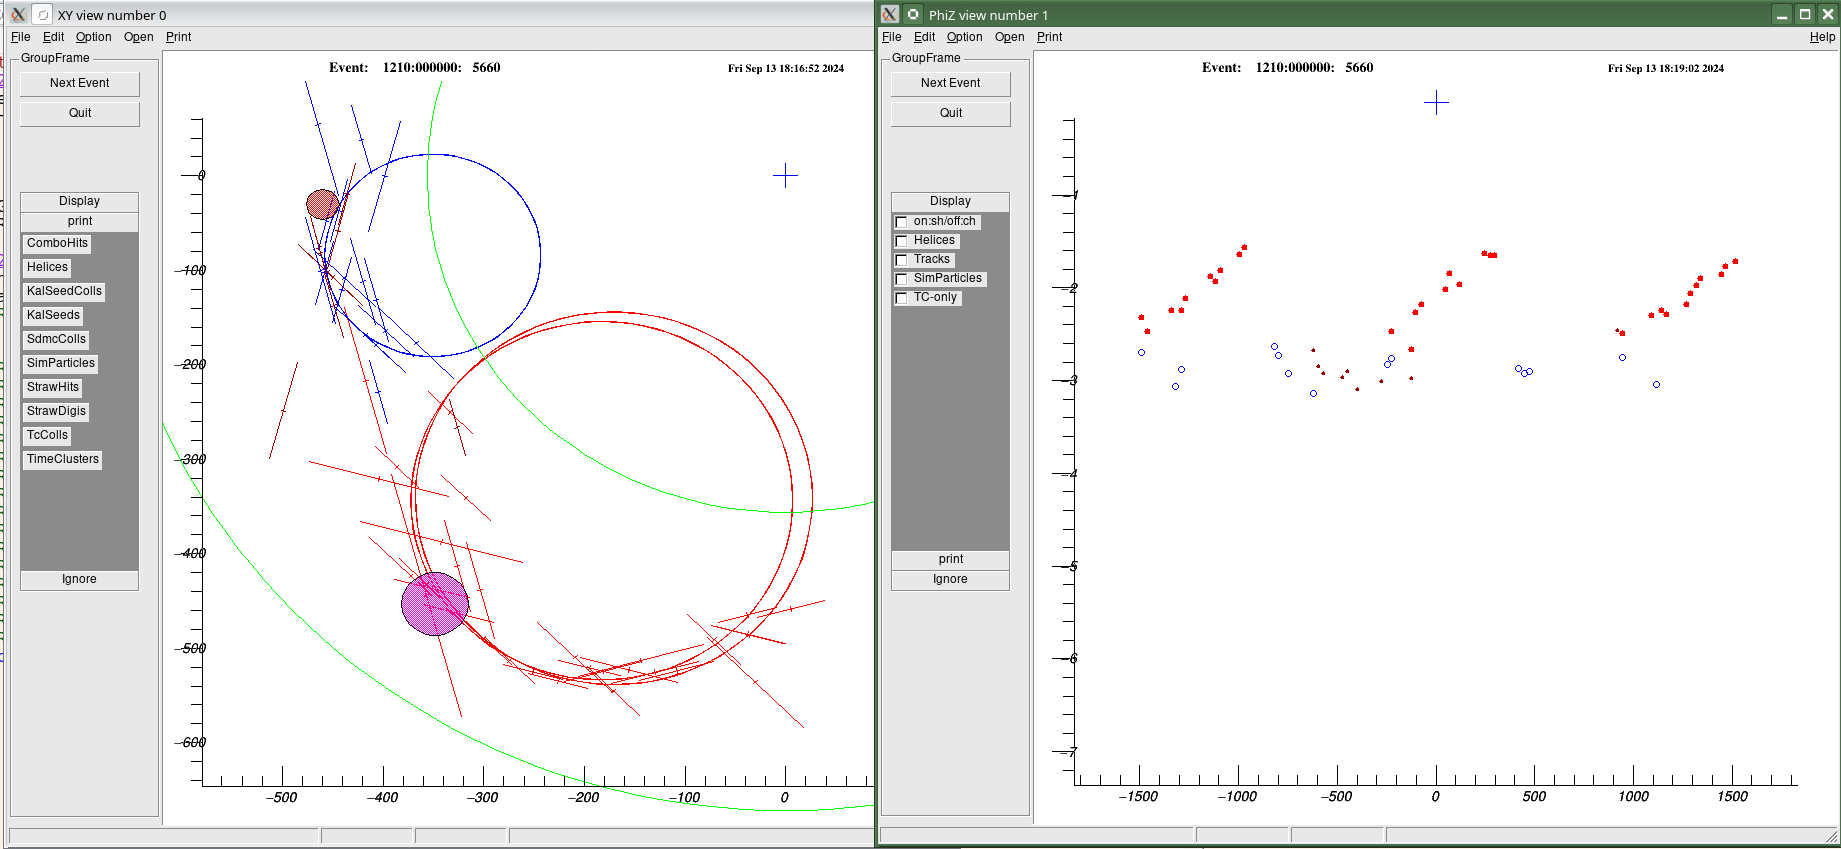
\includegraphics[width=0.95\textwidth]{png/rpc04b0s54r0100_1210_0_005660}
      }
    };
    % \node [text width=8cm, scale=1.0] at (14.5,0.5) {$\mu_B$, expected background mean};
    % \node [text width=8cm, scale=1.0, rotate={90}] at (1.5,7.5) { $S_{D}$, ``discovery'' signal strength  };
  \end{tikzpicture}
  \caption{
    \label{figure:sum_mom_vd13}
    An example of a 129.4 MeV photon conversion event with two tracks
    in the tracker fiducial and only one track (red circle of a smaller radius)
    reconstructed. Shown are the XY and $\phi$-Z event views in the tracker.
    {\red check if some of the positron hits been lost to the delta-electron removal}
  }
  \label{figure:event_display}
\end{figure}


A second type of misreconstruction occurs when hits from both particles are combined to make an unrealistic track with larger radius than either true track. These can occur in place of reconstruction for an individual particle, or in addition to well-reconstructed tracks. Figure~\ref{figure:he_artifact_evts} shows two examples. Taking the sum of momenta for cases with one or more of these combined tracks can significantly overestimate the true total momentum, and results in high energy artifacts out beyond the original RPC photon energy. As part of track reconstruction improvements, better separation of hits between the two tracks will be needed to recover some of these events. 

\begin{figure}[H]
  \begin{tikzpicture}
    \node[anchor=south west,inner sep=0] at (0,0.) {
        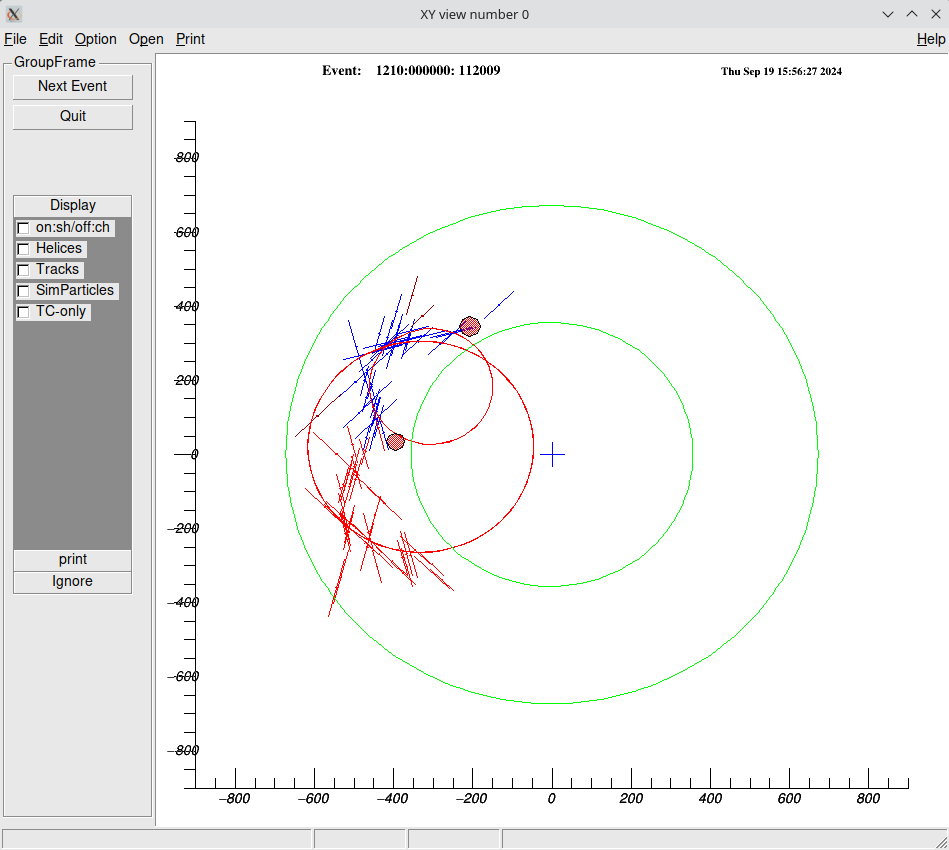
\includegraphics[width=0.54\textwidth]{png/rpc04b0s54r0100_1210_0_112009}
    };
    \node[anchor=south west,inner sep=0] at (9.8,0.) {
        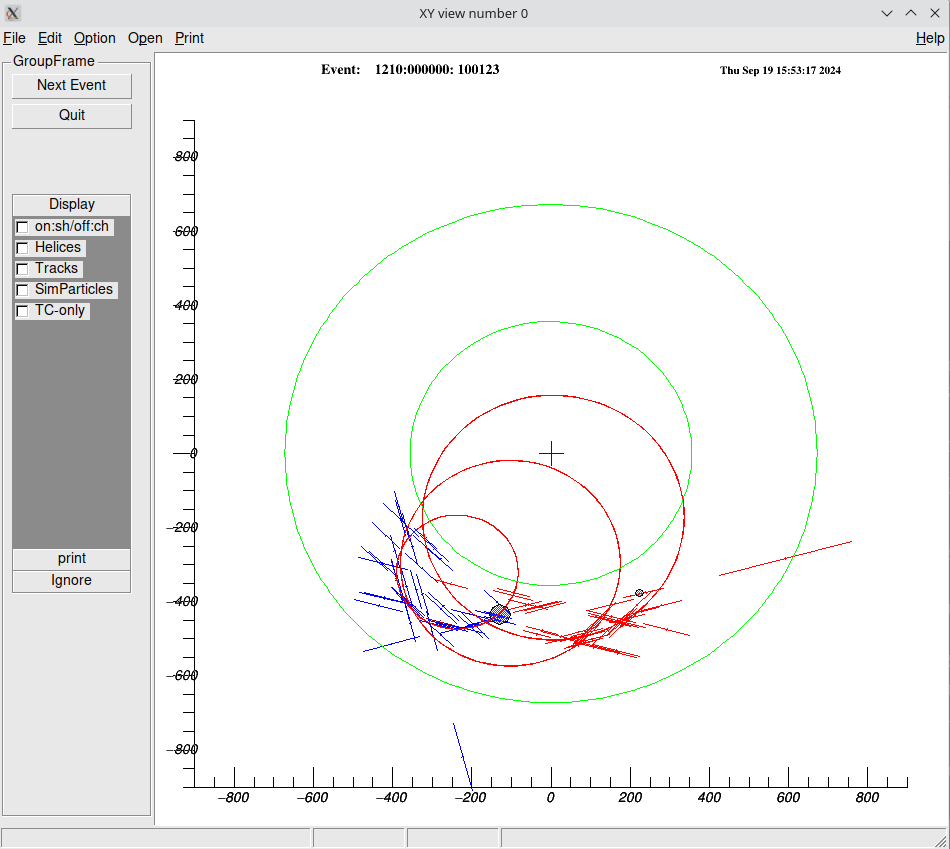
\includegraphics[width=0.54\textwidth]{png/rpc04b0s54r0100_1210_0_100123}
    };
  \end{tikzpicture}
  \caption{
    \label{figure:he_artifact_evts}
   Tracker XY view for two example events where the existing reconstruction combines hits from both electron and positron to make tracks with unrealistic large transverse momentum. Circles include all reconstructed tracks for these events, both artifacts and well-reconstructed tracks (no MC truth tracks are shown here). 
  }
  \label{figure:he_artifact_evts}
\end{figure}


%%% Local Variables:
%%% mode: latex
%%% TeX-master: t
%%% End:
